% ----------------------
\chapter{Nota teórica} 
% ----------------------
\label{C:nota_teorica}

Un robot omnidireccional es una plataforma que se puede mover autonomamente. Son utilizadas en industrias de manufactura flexibles y en ambientes de servicio \cite{Batlle2009}. Hay tres aspectos importantes que posee un robot omnidireccinal. La figura \ref{fig:robot_omnidireccional} ayuda a ilustrar las tres características básicas de un rotot omnidireccional.

A continuación, se procede en las siguientes secciones a clarificar algunos conecptos necesarios para entender cómo se consiguen estas características en un robot móvil.

\begin{figure}[H]
  \centering
  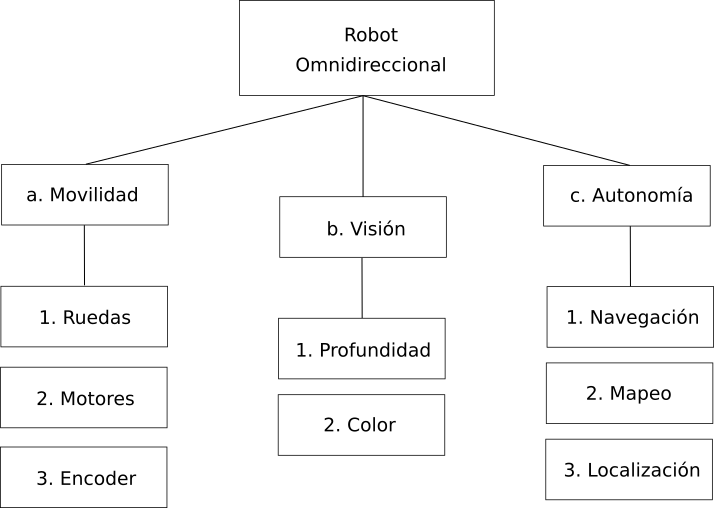
\includegraphics[scale=0.6]{robot_omnidireccional.png}
  \label{fig:robot_omnidireccional}
  \caption{Diagrama de componentes de un robot omnidireccional. Autoría propia.}
\end{figure}


\section{Movilidad}
Existen varios aspectos a considerar cuando se diseña un robot: movilidad, control y posicionamiento. La primera hace referencia a la cantidad de movimientos que un robot puede realizar para llegar a una configuración final. Deben ser capaces de alcanzar cualquier posición y cualquier orientación en su plano de movimiento. Esto quiere decir que el marco del robot debe poseer tres coordenadas independientes del plano general de movimiento \cite{Batlle2009}.

El movimiento se puede realizar con un robot que tiene dos grados de libertad (se puede mover hacia adelante y atrás, con un ángulo de dirección), pero hay que maniobrar. Es más fácil realizar esta tarea si un robot tiene tres grados de libertad. Esto quiere decir, se puede mover hacia adelante y hacia atrás, izquierda derecha, y rotar. De esta manera, la movilidad aumenta, puesto que la cantidad de movimientos posibles que un robot puede realizar para llegar a una configuración final aumenta \cite{Batlle2009}. 


\section{¿A quién va dirigido el trabajo escrito?}
  
Una guía útil para tomar decisiones sobre qué incluir en el trabajo escrito es tener conciencia de cuál es el público meta de la lectura. Esto marca grandes diferencias, pues, por ejemplo, para un sector externo de la carrera habría que iniciar explicando conceptos básicos; mientras que, si está dirigido a profesores, se omite casi todo tema introductorio y se enfoca en los aspectos novedosos del trabajo. Sin embargo, este último enfoque puede dejar a muchos lectores con vacíos importantes de teoría.

Tomando en consideración lo anterior, la recomendación de la Escuela es la siguiente:

\begin{quote}
Los lectores del trabajo escrito del Proyecto Eléctrico son estudiantes de ingeniería eléctrica del último año de carrera.
\end{quote}

Esta recomendación permite tomar algunas decisiones importantes, por ejemplo:

\begin{description}
\item[¿Se debe explicar el concepto de resistencia eléctrica?] No, porque se asume a todo lector familiar con el tema\footnote{A pesar de eso, la explicación de la resistencia eléctrica se ha incluido muchas veces en trabajos escritos.}. Sería justificable cuando el proyecto estudia algún concepto fundamental relacionado con la resistencia.
\end{description}

Como regla de dedo:

\section{``Antecedentes'' vs ``Marco Teórico'' vs ``Estado del Arte''}

\section{Las partes del documento escrito}

\subsection{Asuntos preliminares}

\subsubsection{Portada}

\subsubsection{Hoja de aprobación}

\subsubsection{Resumen}

\subsubsection{Resumen en inglés}

\subsubsection{Dedicatoria}

\subsubsection{Agradecimientos}

\subsubsection{Índices}

\subsection{Cuerpo del documento}

\subsubsection{Primer capítulo: introducción}

\subsubsection{Segundo capítulo: teoría}

\subsection{Contenido posterior}

\subsubsection{Apéndices}

\subsubsection{Bibliografía}

\section{Convenciones básicas de formato en español}

\begin{description}
\item[Mayúsculas en los títulos] Lleva mayúscula solamente la primera letra del título, excepto por nombres propios o siglas que por su naturaleza se escriben en mayúscula.
\end{description}

% Revisar qué hay que dejar de aquí:

\section{Más explicaciones aquí}

En el segundo capítulo del informe, debe resumirse el estudio realizado sobre \emph{estado de la técnica}, en la temática relacionada con el proyecto.  Este se puede denominar ``Antecedentes'', ``Marco de referencia'', ``Base teórica'', o ``Marco teórico''.

Por tratarse de una presentación con base en la recopilación, el análisis y la síntesis de trabajos de otros autores, la referencia adecuada a los mismos, es indispensable.  Toda copia (\emph{¡plagio!}), es inaceptable.

Para indicar las fuentes bibliográficas puede utilizarse el comando del paquete \texttt{natbib} \texttt{\textbackslash cite\{bibtexkey\}} para utilizar el formato ``Autor (año)'' o el comando \texttt{\textbackslash citep\{bibtexkey\}} para mostrarla en el formato ``(Autor, año)''.

%en el siguiente párrafo se supone que se han empleado los comandos cite o citep
Por ejemplo se obtiene: ``Según Wang (1996) la frecuencia ...'' (si se cita con \texttt{cite}), o ``... para este diseño se han utilizado modelos determinísticos (Smith, 2005) y estocásticos (Bell et. al, 2010).''  (si se citan con \texttt{citep}).  

El contenido del capítulo debe ser relevante para el proyecto y no ``material de relleno'', o incluido con el único propósito de ``engordar'' el informe.

El estado de la técnica establece el \emph{punto de partida} del estudio realizado y posiblemente también, la \emph{base de comparación} para las pruebas realizadas.

Este capítulo muestra la capacidad de análisis y síntesis del estudiante.
 
%- declaración de una sección ---------------------------------------
\section{Ecuaciones}
Las ecuaciones estarán centradas y numeradas en forma secuencial por capítulo, al margen derecho.  La referencia a ellas se hará utilizando su número.

¡Texto de ejemplo! - ``El modelo utilizado para representar al proceso, es de primer orden más tiempo muerto, dado por la función de transferencia

\begin{equation}  %inclusión de ecuaciones
	P(s) = \frac{K \me^{-Ls}}{Ts+1}, \label{ec:01}
\end{equation}

\noindent donde $K$ es la ganancia, $T$ la ...''  
%si el texto después de la ecuación no inicia un nuevo párrafo y se ha insertado una linea en blanco depues de esta, es necesario poner \noindent para que el texto siguiente no tenga sangría (formato predeterminado).

Las ecuaciones forman parte del texto, por lo que deben terminarse con el signo de puntuación requerido, una coma o un punto.

Para referirse a ellas se hace uso de la etiqueta (\texttt{label}) asignada a la ecuación usando \texttt{\textbackslash eqref\{etiqueta\}} que mostrará su número.  Por ejemplo ``El modelo \eqref{ec:01} es el más utilizado para ...''

%en el siguiente párrafo se supone que se ha utilizado \eqref{etiqueta} para referencias las ecuacioenes
El texto debe mostrar ``... sustituyendo (2.4) y (2.5) en (2.2), se obtiene ...'' y no ``... sustituyendo la ecuación (2.4) y la ecuación (2.5) en la ecuación (2.2), se obtiene...''  

¡Ejemplos de ecuaciones!

Usando \texttt{equation}:
\begin{equation}
	\tau \frac{\md T_{tc}(t)}{\md t} + T_{tc}(t) = T_{gas}(t).
\end{equation}

Ecuaciones alineadas utilizando \texttt{align}:

\begin{align}
	L_1 \frac{\md i_{L_1} (t)}{\md t} &= v(t) - R_1 i_{L_1}(t) - v_c(t), \\
	C \frac{\md v_c (t)}{\md t} &= i_L(t)- \frac{1}{R_2} v_c(t).
\end{align}

\section{Figuras y cuadros}
Las figuras y los cuadros son \emph{elementos flotantes}. Aunque se le puede ``sugerir'' a \LaTeX~ donde ubicarlos, es conveniente dejarlos ``flotar''.

\subsection{Figuras}
Las referencias a las figuras debe hacerse utilizando el número asignado a ellas.  Para esto se le asigna una etiqueta (con \texttt{label}) y luego se utiliza esta para hacer la referencia (con \texttt{ref}).  Usar en el texto el término ``figura'' y no Fig.'' o ``fig.''.

La leyenda (con \texttt{caption}) de la figura, irá en la parte inferior de la misma.  Como en forma predeterminada en la clase \texttt{eieproyecto} las figuras están centradas, no es necesario usar \texttt{centering} para hacerlo.

Por ejemplo ``Considérese el diagrama de bloques mostrado en la figura en donde el proceso controlado está dado por ...''.

No utilizar ``... en la siguiente figura ...'', emplear siempre el número correspondiente para referirse a ellas.

Cuando las figuras son muy pequeñas, se puede colocar la leyenda al lado de la misma, con el ambiente \texttt{SCfigure} del paquete \texttt{sidecap}.  Un ejemplo de esto se muestra en la figura.

Cuando un gráfico muestre varias curvas, estas deben poderse distinguir, no solamente en la pantalla de la computadora, usando diferentes colores, si no también en una impresión en blanco y negro, utilizando lineas de trazos diferentes, como se muestra en la figura.

\LaTeX~ nunca coloca las figuras y los cuadros en una página anterior a la en que son incluidas.  Los elementos flotantes los coloca en la página donde se hace referencia a ellos, o en una de las siguientes.

Además, en el texto debe hacerse referencia a todas las figuras y cuadros incluidos en el informe.  Si alguno de ellos no se menciona en el texto, es que no se requiere para entender el desarrollo presentado y por lo tanto es innecesario y se podría omitir sin que se afecte el informe.

\subsection{Cuadros}
Los cuadros son el otro elemento flotante utilizado en los informes y también es conveniente dejar que \LaTeX~ los coloque en donde considere que es más adecuado.

Los cuadros no llevarán ninguna línea divisoria vertical, solo horizontales. Una en la parte superior (\texttt{toprule}), una bajo la línea de cabecera (\texttt{midrule}) y una en la parte inferior (\texttt{bottomrule}).  Normalmente basta con estas tres líneas, pero si fuera necesaria alguna otra para una división horizontal, esta debe ser del tipo \texttt{midrule}.

Se recomienda revisar los comandos para la construcción de cuadros, incluidos en el manual de la clase \texttt{memoir} \cite{memoir2011}, o en la del paquete \texttt{booktabs} \cite{fear2005}.

La leyenda (\texttt{caption}) del cuadro se mostrará en la parte superior.  Para poder referirse al cuadro (con \texttt{ref}), se le asigna una etiqueta (con \texttt{label}).

En forma predefinida, los cuadros se mostrarán centrados horizontalmente, por lo que no es necesario hacer esa indicación. 

El cuadro \ref{tab:01} es un ejemplo de un cuadro de datos simple.

%inclusión de un cuadro con datos
\begin{table}
\caption{Parámetros de los modelos.} \label{tab:01o}
		\begin{tabular}{@{}*{4}{c}@{}}
    \toprule
    $K_p$ & $T_1$ & $T_2$ & $L$ \\
    \midrule
     1,01 & 1,50 & 0,75 & 0,12 \\
		 1,15 & 2,37 & 0,15 & 0,28 \\
		 2,25 & 5,89 & 2,15 & 1,60 \\
    \bottomrule
    \end{tabular}
\end{table}

Si la primera columna corresponde a leyendas o parámetros que identifican los datos de la línea, esta debe estar justificada a la izquierda, como se muestra en el cuadro \ref{tab:AH}, que ha sido tomada de \cite{astromhagglund2006}.

\begin{table}
\caption{Parámetros de los controladores ...} \label{tab:AH}
\begin{center}
    \begin{tabular}{@{}l*{7}{c}@{}}
    \toprule
    Controller & $K$ & $K_i$ & $K_d$ & $\beta$ & $T_i$ & $T_d$ & IAE \\
    \midrule
    PD &  1,333 & 0 & 1,333 & 1 & 0 &1 & $\infty$ \\
		PI & 0,433 & 0,192 & 0 & 0,14 & 2,25 & 0 & 6,20 \\
		PID MIGO & 1,305 & 0,758 & 1,705 & 0 & 1,72 & 1,31 & 2,25 \\
		PID $T_i=4 \ T_d$ & 1,132 & 0,356 & 0,900 & 0,9 & 3,18 & 0,80 & 2,51 \\
    \bottomrule
    \end{tabular}
\end{center}
\end{table}

Se puede especificar una cabecera para más de una columna y utilizar lineas horizontales que abarquen solo unas pocas columnas, como se muestra en el cuadro \ref{tab:muestra}.

\begin{table}
\caption{Ejemplo de otro cuadro.} \label{tab:muestra}
	\begin{tabular}{@{}l*{4}{c}@{}}
	\toprule
	& \multicolumn{2}{c}{Prueba 1} & \multicolumn{2}{c}{Prueba 2} \\
	\cmidrule(l{2pt}r{2pt}){2-3}\cmidrule(l{2pt}r{2pt}){4-5} 
	& $\Delta E=5$ V & $\Delta E = -5$ V & $\Delta E = 10$ V & $\Delta E = -10$ V \\
	\midrule
	Ganancia             &  1,06 & 0,98 & 1,12 & 0,97 \\
	Tiempo subida, s  &  5,67 & 5,89 & 6,02 & 5,74 \\
	Sobrepaso máx, \%        &  2,67 & 3,25 & 2,91 & 1,56 \\
	Error, \% &  0,25 & 0,56 & 0,97 & 0,18 \\
	\bottomrule
	\end{tabular}
\end{table}

\newpage
Cuando los cuadros son pequeños (abarcan menos de la mitad del ancho del texto), se puede colocar la leyenda a la par del cuadro, utilizando el ambiente \texttt{SCtable} del paquete \texttt{sidecap}, tal como se muestra en el cuadro \ref{tab:01}.  Compare este, con el cuadro \ref{tab:01o}.

\begin{SCtable}
\caption[Parámetros de los modelos]{Parámetros de los modelos, obtenidos a partir de las tres curvas de reacción.} \label{tab:01}
    \begin{tabular}{@{}*{4}{c}@{}}
    \toprule
    $K_p$ & $T_1$ & $T_2$ & $L$ \\
    \midrule
     1,01 & 1,50 & 0,75 & 0,12 \\
		 1,15 & 2,37 & 0,15 & 0,28 \\
		 2,25 & 5,89 & 2,15 & 1,60 \\
    \bottomrule
    \end{tabular}
\end{SCtable}
